\lab{The SVD and Image Compression}{The SVD and Image Compression}
\label{lab:SVD}
\objective{The Singular Value Decomposition (SVD) is an incredibly useful matrix factorization that is widely used in both theoretical and applied mathematics.
The SVD is structured in a way that makes it easy to construct low-rank approximations of matrices, and it is therefore the basis of several data compression algorithms.
In this lab we learn to compute the SVD and use it to implement a simple image compression routine.
}

\begin{comment} % Vague motivation, most of which is in the book.
The \emph{Singular Value Decomposition} or \emph{SVD} is a matrix decomposition that is widely used in both theoretical and applied mathematics.
Originally discovered by theoretical mathematicians, it is a canonical way to decompose a matrix.
Its practical use became apparent later on when Erhard Schmidt showed that the SVD could be a computational tool for providing low-rank matrix approximations.
Modern developments continue to confirm the importance of the SVD in both computational and theoretical applications.

The theoretical use of the \emph{Singular Value Decomposition} or \emph{SVD} has long been appreciated.
In fact, the idea of a canonical way of decomposing a matrix was so alluring that the SVD was independently discovered by at least four people through use of both  integral equations and systems of linear equations.

However, it wasn't until Erhard Schmidt showed how the SVD could be a computational tool for providing low-rank approximations that the practical applications became apparent.
Since Schmidt's work, further developments have confirmed the importance of the SVD in both computational and theoretical applications.
\end{comment}

\begin{comment} % Historical background, super overkill.
The \emph{Singular Value Decomposition} is so important that it was discovered multiple times by different people in different ways.
The foundation work in systems of linear equations was laid by Gauss and Cauchy in the 1820's and later by Jacobi in 1846 with his work with the LU decomposition; however, the real work with the SVD started with Eugenio Beltrami.
In a paper he published in 1873 he was the first to work with the SVD; he was limited to real, square, nonsingular matrices with distinct singular values.
A year later, Camille Jordan published his own independent work that was more rigorous and avoided some of the pitfalls of Beltrami's research.
Together, Beltrami and Jordan are considered the co-discoverers of the singular value decomposition.

Later, James Joseph Sylvester independently presented an iterative algorithm and a rule for carrying out the reduction in 1889.
This rule was essentially Beltrami's work.
However Sylvester sent the note detailing his rule to the same journal Jordan had published in, showing not just his ignorance of Jordan's and Beltrami's works but his perception of the importance of the SVD.

The concurrent and independent derivation of the SVD shows its importance as a theoretical tool, but it wasn't until Erhard Schmidt discovered a computational use for the SVD that the practical applications became apparent.
Schmidt used integral equations rather than linear equations to derive the SVD, but his most important contribution was showing how the SVD could be a computational tool to obtain optimal, low-rank approximations.

Since Schmidt's work, further developments have confirmed the importance of the SVD in both practical and theoretical applications.
\end{comment}

The SVD of a matrix $A$ is a factorization $A = U \Sigma V\hrm$ where $U$ and $V$ have orthonormal columns and $\Sigma$ is diagonal.
The diagonal entries of $\Sigma$ are called the \emph{singular values} of $A$ and are the square roots of the eigenvalues of $A\hrm A$.
Since $A\hrm A$ is always positive semidefinite, its eigenvalues are all real and nonnegative, so the singular values are also real and nonnegative.
The singular values $\sigma_i$ are usually sorted in decreasing order so that $ \Sigma = \mbox{diag}(\sigma_1,\sigma_2,\ldots,\sigma_n)$ with $\sigma_1 \geq \sigma_2 \geq \ldots \geq \sigma_n \geq 0$.
The columns $\mathbf{u}_i$ of $U$, the columns $\mathbf{v}_i$ of $V$, and the singular values of $A$ satisfy $A\mathbf{v}_i = \sigma_i \mathbf{u}_i$.

Every $m\times n$ matrix $A$ of rank $r$ has an SVD with exactly $r$ nonzero singular values.
Like the QR decomposition, the SVD has two main forms.
\begin{itemize}
    \item \textbf{Full SVD}: Denoted $A = U\Sigma V\hrm$.
    $U$ is $m\times m$, $V$ is $n\times n$, and $\Sigma$ is $m\times n$.
    The first $r$ columns of $U$ span $\mathscr{R}(A)$, and the remaining $n -r$ columns span $\mathscr{N}(A\hrm)$.
    Likewise, the first $r$ columns of $V$ span $\mathscr{R}(A\hrm)$, and the last $m - r$ columns span $\mathscr{N}(A)$.
    \item \textbf{Compact (Reduced) SVD}: Denoted $A = U_1\Sigma_1 V\hrm_1$.
    $U_1$ is $m\times r$ (the first $r$ columns of $U$), $V_1$ is $n \times r$ (the first $r$ columns of $V$), and $\Sigma_1$ is $r\times r$ (the first $r\times r$ block of $\Sigma$).
    This smaller version of the SVD has all of the information needed to construct $A$ and nothing more.
    The zero singular values and the correpsonding columns of $U$ and $V$ are neglected.
\end{itemize}
%
\begin{align*} % Full and compace SVD.
\begin{array}{cccc}
\textcolor{red}{U_1\ (m \times r)} & \textcolor{blue}{\Sigma_1\ (r \times r)} & \textcolor{green}{V\hrm_1\ (r \times n)} \\ \\
\left[\begin{array}{ccccccc}
\arrayrulecolor{red}
\cline{2-4}
& \lvl{}     &        & \rvl{}     &          &        &      \\
& \lvl{}     &        & \rvl{}     &          &        &      \\
& \lvl{}     &        & \rvl{}     &          &        &      \\
& \lvl{\u_1} & \cdots & \rvl{\u_r} & \u_{r+1} & \cdots & \u_m \\
& \lvl{}     &        & \rvl{}     &          &        &      \\
& \lvl{}     &        & \rvl{}     &          &        &      \\
& \lvl{}     &        & \rvl{}     &          &        &      \\
\cline{2-4}
\end{array}\right]
&
\left[\begin{array}{cccccccc}
\arrayrulecolor{blue}
\cline{2-4}
& \lvl{\sigma_{1}}  &   & \rvl{}         &   &        &   \\
& \lvl{}       & \ddots & \rvl{}         &   &        &   \\
& \lvl{}       &        & \rvl{\sigma_{r}} & &        &   \\
\cline{2-4}
&              &        &                & 0 &        &   \\
&              &        &                &   & \ddots &   \\
&              &        &                &   &        & 0 \\
\end{array}\right]
&
\left[\begin{array}{ccccccc}
\arrayrulecolor{green}
\cline{2-6}
& \lvl{} & & \v\hrm_1 & & \rvl{} & \\
& \lvl{} & & \vdots   & & \rvl{} & \\
& \lvl{} & & \v\hrm_r & & \rvl{} & \\
\cline{2-6}
& & & \v\hrm_{r+1} & & & \\
& & & \vdots       & & & \\
& & & \v\hrm_n     & & & \\
\end{array}\right]
\\ \\
U\ (m \times m) & \Sigma\ (m \times n) & V\hrm (n \times n) \\
\end{array}
\end{align*}

Finally, the SVD yields an \emph{outer product expansion} of $A$ in terms of the singular values and the columns of $U$ and $V$,
\begin{equation}
\label{eq:svd-outer-product}
A = \sum_{i=1}^r \sigma_i\u_i\v\hrm_i.
\end{equation}
Note that only terms from the compact SVD are needed for this expansion.

\subsection*{Computing the Compact SVD} % -------------------------------------

It is difficult to compute the SVD from scratch because it is an eigenvalue-based decomposition.
However, given an eigenvalue solver such as \li{scipy.linalg.eig()}, the algorithm becomes much simpler.
First, obtain the eigenvalues and eigenvectors of $A\hrm A$, and use these to compute $\Sigma$.
Since $A\hrm A$ is normal, it has an orthonormal eigenbasis, so set the columns of $V$ to be the eigenvectors of $A\hrm A$.
Then, since $A\v_i = \sigma_i \u_i$, construct $U$ by setting its columns to be $\u_i = \frac{1}{\sigma_i}A\v_i$.

The key is to sort the singular values and the corresponding eigenvectors in the same manner.
In addition, it is computationally inefficient to keep track of the entire matrix $\Sigma$ since it is a matrix of mostly zeros, so we need only store the singular values as a vector $\boldsymbol{\sigma}$.
The entire procedure for computing the compact SVD is given below.
% For the compact SVD, keep all of the nonzero singular values.
% For the truncated SVD, keep only the largest $k$.

\begin{algorithm} % Compact SVD.
\begin{algorithmic}[1]
\Procedure{compact\_SVD}{$A$}
\State $\boldsymbol{\lambda}, V \gets$ eig$(A\hrm A)$
    \Comment{Calculate the eigenvalues and eigenvectors of $A\hrm A$.}
\State $\boldsymbol{\sigma} \gets \sqrt{\boldsymbol{\lambda}}$
    \Comment{Calculate the singular values of $A$.}
\State $\boldsymbol{\sigma} \gets$ sort$(\boldsymbol{\sigma})$
    \Comment{Sort the singular values \textbf{from greatest to least}.}
    \label{step:sort-singular-values}
\State $V \gets$ sort($V$)
    \Comment{Sort the eigenvectors \textbf{the same way} as in the previous step.}
\State $r \gets $ count($\boldsymbol{\sigma} \ne 0)$
    \Comment{Count the number of nonzero singular values (the rank of $A$).}
    \label{step:nonzero-singular-values}
\State $\boldsymbol{\sigma}_1 \gets \boldsymbol{\sigma}_{:r}$
    \Comment{Keep only the positive singular values.}
\State $V_1 \gets V_{:,:r}$
    \Comment{Keep only the corresponding eigenvectors.}
\State $U_1 \gets AV_1 / \boldsymbol{\sigma}_1$
    \Comment{Construct $U$ with array broadcasting.}
    \label{step:SVD-construct-U}
\State \pseudoli{return} $U_1, \boldsymbol{\sigma}_1, V\hrm_1$
\EndProcedure
\caption{}
\label{alg:compact-svd}
\end{algorithmic}
\end{algorithm}

\begin{problem} % Compute the compact SVD.
Write a function that accepts a matrix $A$ and a small error tolerance \li{tol}.
Use Algorithm \ref{alg:compact-svd} to compute the compact SVD of $A$.
In step \ref{step:nonzero-singular-values}, compute $r$ by counting the number of singular values that are greater than \li{tol}.

Consider the following tips for implementing the algorithm.
\begin{itemize}
    \item The Hermitian $A\hrm$ can be computed with \li{A.conj().T}.
    \item In step \ref{step:sort-singular-values}, the way that $\boldsymbol{\sigma}$ is sorted needs to be stored so that the columns of $V$ can be sorted the same way.
    Consider using \li{np.argsort()} and fancy indexing to do this, but remember that by default it sorts from least to greatest (not greatest to least).
    \item Step \ref{step:SVD-construct-U} can be done by looping over the columns of $V$, but it can be done more easily and efficiently with array broadcasting.
\end{itemize}

Test your function by calculating the compact SVD for random matrices.
Verify that $U$ and $V$ are orthonormal, that $U\Sigma V\hrm = A$, and that the number of nonzero singular values is the rank of $A$.
You may also want to compre your results to SciPy's SVD algorithm.
%
\begin{lstlisting}
>>> import numpy as np
>>> from scipy import linalg as la

# Generate a random matrix and get its compact SVD via SciPy.
>>> A = np.random.random((10,5))
>>> U,s,Vh = la.svd(A, full_matrices=False)
>>> print(U.shape, s.shape, Vh.shape)
(10, 5) (5,) (5, 5)

# Verify that U is orthonormal, U Sigma Vh = A, and the rank is correct.
>>> np.allclose(U.T @ U, np.identity(5))
<<True>>
>>> np.allclose(U @ np.diag(s) @ Vh, A)
<<True>>
>>> np.linalg.matrix_rank(A) == len(s)
<<True>>
\end{lstlisting}
\label{prob:calculate-compact-svd}
\end{problem}

\subsection*{Visualizing the SVD} % -------------------------------------------

An $m\times n$ matrix $A$ defines a linear transformation that sends points from $\mathbb{R}^n$ to $\mathbb{R}^m$.
The SVD decomposes a matrix into two rotations and a scaling, so that any linear transformation can be easily described geometrically.
Specifically, $V\hrm$ represents a rotation, $\Sigma$ a rescaling along the principal axes, and $U$ another rotation.

\begin{figure}
\centering
\begin{subfigure}{.35\textwidth}
  \centering
  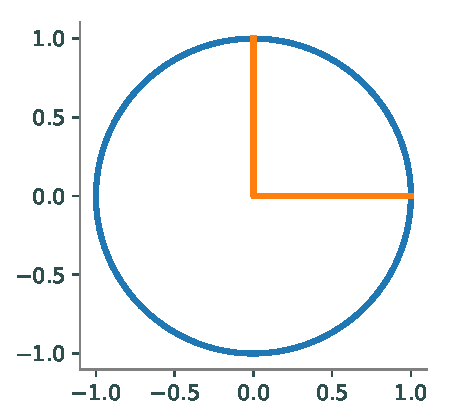
\includegraphics[width=\textwidth]{figures/unit_circle.pdf}
  \caption{$S$}
\end{subfigure}
\quad
\begin{subfigure}{.35\textwidth}
  \centering
  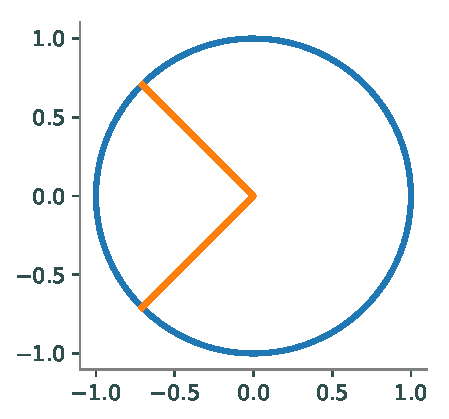
\includegraphics[width=\textwidth]{figures/vcircle.pdf}
  \caption{$V\hrm S$}
\end{subfigure}
\\
\begin{subfigure}{.35\textwidth}
  \centering
  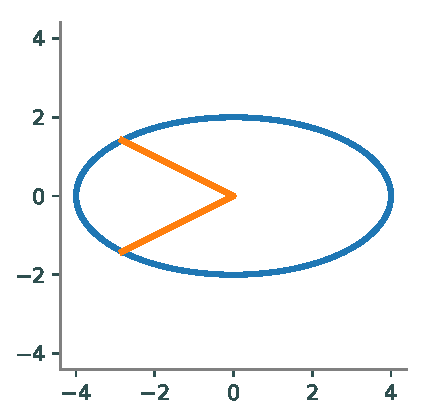
\includegraphics[width=\textwidth]{figures/svcircle.pdf}
  \caption{$\Sigma V\hrm S$}
\end{subfigure}
\quad
\begin{subfigure}{.35\textwidth}
  \centering
  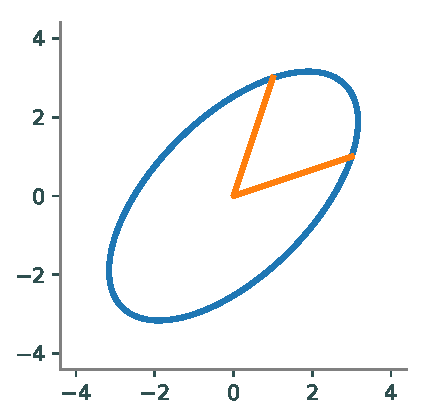
\includegraphics[width=\textwidth]{figures/full_transformation.pdf}
  \caption{$U \Sigma V\hrm S$}
\end{subfigure}
\caption{Each step in transforming the unit circle and two unit vectors using the matrix $A$.}
\label{fig:svd-visualization}
\end{figure}

\begin{problem} % Visualize the SVD.
Write a function that accepts a $2 \times 2$ matrix $A$.
Generate a $2 \times 200$ matrix $S$ representing a set of 200 points on the unit circle, with $x$-coordinates on the top row and $y$-coordinates on the bottom row (recall the equation for the unit circle in polar coordinates:
$x = \cos(\theta)$, $y = \sin(\theta)$, $\theta\in[0,2\pi]$).
Also define the matrix
\[
E =
\left[\begin{array}{c|c|c}
\arrayrulecolor{gray}
\e_1 & \0 & \e_2
\end{array}\right]
=
\left[\begin{array}{ccc} 1 & 0 & 0 \\ 0 & 0 & 1 \end{array}\right],
\]
so that plotting the first row of $S$ against the second row of $S$ displays the unit circle, and plotting the first row of $E$ against its second row displays the standard basis vectors in $\mathbb{R}^2$.

Compute the full SVD $A = U\Sigma V\hrm$ using \li{scipy.linalg.svd()}.
Plot four subplots to demonstrate each step of the transformation, plotting $S$ and $E$, $V\hrm S$ and $V\hrm E$, $\Sigma V\hrm S$ and $\Sigma V\hrm E$, then $U\Sigma V\hrm S$ and $U \Sigma V\hrm E$.

For the matrix \[A =  \left[\begin{array}{cc}3 & 1\\1 & 3\end{array}\right],\]
your function should produce Figure \ref{fig:svd-visualization}.
\\
(Hint: Use \li{plt.axis("equal")} to fix the aspect ratio so that the circles don't appear elliptical.)
\end{problem}

\begin{comment}
\subsection*{Image Data Compression}
In this lab, we explore how the SVD can be used to compress image data.
Recall that an image is simply a matrix where each position is the color value for the pixel in that position.
The SVD lets us choose how much information to keep, and what information is most important.
Larger eigenvalues correspond to columns of $U$ and $V$ that contain more information, while smaller eigenvalues correspond to less important columns.
This idea is used in many areas of applied mathematics including signal processing, statistics, semantic indexing (search engines), and control theory.
\end{comment}

\section*{Using the SVD for Data Compression} % ===============================

\subsection*{Low-Rank Matrix Approximations} % --------------------------------

If $A$ is a $m\times n$ matrix of rank $r < \min\{m,n\}$, then the compact SVD offers a way to store $A$ with less memory.
Instead of storing all $mn$ values of $A$, storing the matrices $U_1$, $\Sigma_1$ and $V_1$ only requires saving a total of $mr+r+nr$ values.
For example, if $A$ is $100 \times 200$ and has rank $20$, then $A$ has $20,000$ values, but its compact SVD only has total $6,020$ entries, a significant decrease.

The \emph{truncated SVD} is an approximation to the compact SVD that allows even greater efficiency at the cost of a little accuracy.
Instead of keeping all of the nonzero singular values, the truncated SVD only keeps the first $s < r$ singular values, plus the corresponding columns of $U$ and $V$.
In this case, (\ref{eq:svd-outer-product}) becomes
\begin{equation*}
A_s = \sum_{i=1}^s \sigma_i\u_i\v\hrm_i.
\end{equation*}

More precisely, the truncated SVD of $A$ is $A_s = \widehat{U}\widehat{\Sigma} \widehat{V}\hrm$, where
$\widehat{U}$ is $m\times s$, $\widehat{V}$ is $n \times s$, and $\widehat{\Sigma}$ is $s\times s$.
The resulting matrix $A_s$ has rank $s$ and is only an approximation to $A$, since $r - s$ nonzero singular values are neglected.

\begin{align*} % Compact and truncated SVD.
\begin{array}{cccc}
\textcolor{red}{\widehat{U}\ (m \times s)} & \textcolor{blue}{\widehat{\Sigma}\ (s \times s)} & \textcolor{green}{\widehat{V}\hrm\ (s \times n)} \\
\left[\begin{array}{ccccccc}
\arrayrulecolor{red}
\cline{2-4}
& \lvl{}     &        & \rvl{}     &          &        &      \\
& \lvl{}     &        & \rvl{}     &          &        &      \\
& \lvl{}     &        & \rvl{}     &          &        &      \\
& \lvl{\u_1} & \cdots & \rvl{\u_s} & \u_{s+1} & \cdots & \u_r \\
& \lvl{}     &        & \rvl{}     &          &        &      \\
& \lvl{}     &        & \rvl{}     &          &        &      \\
& \lvl{}     &        & \rvl{}     &          &        &      \\
\cline{2-4}
\end{array}\right]
&
\left[\begin{array}{cccccccc}
\arrayrulecolor{blue}
\cline{2-4}
& \lvl{\sigma_{1}}  &   & \rvl{}         &   &        &   \\
& \lvl{}       & \ddots & \rvl{}         &   &        &   \\
& \lvl{}       &        & \rvl{\sigma_{s}} & &        &   \\
\cline{2-4}
&              &        &                & \sigma_{s+1} &        &   \\
&              &        &                &   & \ddots &   \\
&              &        &                &   &        & \sigma_r \\
\end{array}\right]
&
\left[\begin{array}{ccccccc}
\arrayrulecolor{green}
\cline{2-6}
& \lvl{} & & \v\hrm_1 & & \rvl{} & \\
& \lvl{} & & \vdots   & & \rvl{} & \\
& \lvl{} & & \v\hrm_s & & \rvl{} & \\
\cline{2-6}
& & & \v\hrm_{s+1} & & & \\
& & & \vdots       & & & \\
& & & \v\hrm_r     & & & \\
\end{array}\right]
\\
U_1\ (m \times r) & \Sigma_1\ (r \times r) & V\hrm_1 (r \times n) \\
\end{array}
\end{align*}

The beauty of the SVD is that it makes it easy to select the information that is most important.
Larger singular values correspond to columns of $U$ and $V$ that contain more information, so dropping the smallest singular values retains as much information as possible.
In fact, given a matrix $A$, its rank-$s$ truncated SVD approximation $A_s$ is the \emph{best rank $s$ approximation} of $A$ with respect to both the induced 2-norm and the Frobenius norm.
This result is called the \emph{Schmidt, Mirsky, Eckhart-Young theorem}, a very significant concept that appears in signal processing, statistics, machine learning, semantic indexing (search engines), and control theory.

\begin{comment}
We can also calculate $A_s$ by finding the full SVD, and setting all singular values after the $k$th to zero.
Thus the modified $\Sigma$ would be
\begin{equation*}
\Sigma_{s} = \mbox{diag}(\sigma_1,\sigma_2,\ldots,\sigma_s,0,\ldots,0).
\end{equation*}
Multiplying this matrix with the original $U$ and $V\hrm$ will give the same $A_s$ that was found by computing the truncated SVD directly.
\end{comment}

\begin{problem} % Lowest-rank approximation.
Write a function that accepts a matrix $A$ and a positive integer $s$.
\begin{enumerate}
\item Use your function from Problem \ref{prob:calculate-compact-svd} or \li{scipy.linalg.svd()} to compute the compact SVD of $A$, then form the truncated SVD by stripping off the appropriate columns and entries from $U_1$, $\Sigma_1$, and $V_1$.
Return the best rank $s$ approximation $A_s$ of $A$ (with respect to the induced 2-norm and Frobenius norm).
\item Also return the number of entries required to store the truncated form $\widehat{U}\widehat{\Sigma} \widehat{V}\hrm$ (where $\widehat{\Sigma}$ is stored as a one-dimensional array, not the full diagonal matrix).
The number of entries stored in NumPy array can be accessed by its \li{size} attribute.
\begin{lstlisting}
>>> A = np.random.random((20, 20))
>>> A.size
400
\end{lstlisting}
\item If $s$ is greater than the number of nonzero singular values of $A$ (meaning $s > $ rank$(A)$), raise a \li{ValueError}.
\end{enumerate}
Use \li{np.linalg.matrix_rank()} to verify the rank of your approximation.
% , and verify that the number of entries required is equal to $ms + s + ns$.
\label{prob:svd_approx}
\end{problem}

\subsection*{Error of Low-Rank Approximations} % ------------------------------

Another result of the Schmidt, Mirsky, Eckhart-Young theorem is that the exact 2-norm error of the best rank-$s$ approximation $A_s$ for the matrix $A$ is the $(s+1)$th singular value of $A$:
\begin{equation}
\label{eq:svd-approximation-error}
\|A - A_s\|_2 = \sigma_{s+1}.
\end{equation}
%
This offers a way to approximate $A$ within a desired error tolerance $\epsilon$:
choose $s$ such that $\sigma_{s+1}$ is the largest singular value that is less than $\epsilon$, then compute $A_s$.
This $A_s$ throws away as much information as possible without violating the property $\|A - A_s\|_2 < \epsilon$.

\begin{problem} % Lowest Rank Approximation
Write a function that accepts a matrix $A$ and an error tolerance $\epsilon$.
\begin{enumerate}
\item Compute the compact SVD of $A$, then use (\ref{eq:svd-approximation-error}) to compute the lowest rank approximation $A_s$ of $A$ with 2-norm error less than $\epsilon$.
Avoid calculating the SVD more than once.
\\ (Hint: \li{np.argmax()}, \li{np.where()}, and/or fancy indexing may be useful.)
\item As in the previous problem, also return the number of entries needed to store the resulting approximation $A_s$ via the truncated SVD.
\item If $\epsilon$ is less than or equal to the smallest singular value of $A$, raise a \li{ValueError}; in this case, $A$ cannot be approximated within the tolerance by a matrix of lesser rank.
\end{enumerate}
This function should be close to identical to the function from Problem \ref{prob:svd_approx}, but with the extra step of identifying the appropriate $s$.
Construct test cases to validate that $\| A - A_s \|_2 < \epsilon$.
\end{problem}

\subsection*{Image Compression} % ---------------------------------------------

Images are stored on a computer as matrices of pixel values.
Sending an image over the internet or a text message can be expensive, but computing and sending a low-rank SVD approximation of the image can considerably reduce the amount of data sent while retaining a high level of image detail.
Successive levels of detail can be sent after the inital low-rank approximation by sending additional singular values and the corresponding columns of V and U.

% TODO: redo the numbers in this paragraph for the full hubble image.
Examining the singular values of an image gives us an idea of how low-rank the approximation can be.
Figure \ref{fig:hubble} shows the image in \texttt{hubble\_gray.jpg} and a log plot of its singular values.
The plot in \ref{fig:hubble-log-svals} is typical for a photograph---the singular values start out large but drop off rapidly.
In this rank $1041$ image, $913$ of the singular values are $100$ or more times smaller than the largest singular value.
By discarding these relatively small singular values, we can retain all but the finest image details, while storing only a rank $128$ image.
This is a \textbf{huge} reduction in data size.

\begin{figure}[H] % Hubble image + plot of singular values.
\captionsetup[subfigure]{justification=centering}
\centering
\begin{subfigure}{.49\textwidth}
    \centering
    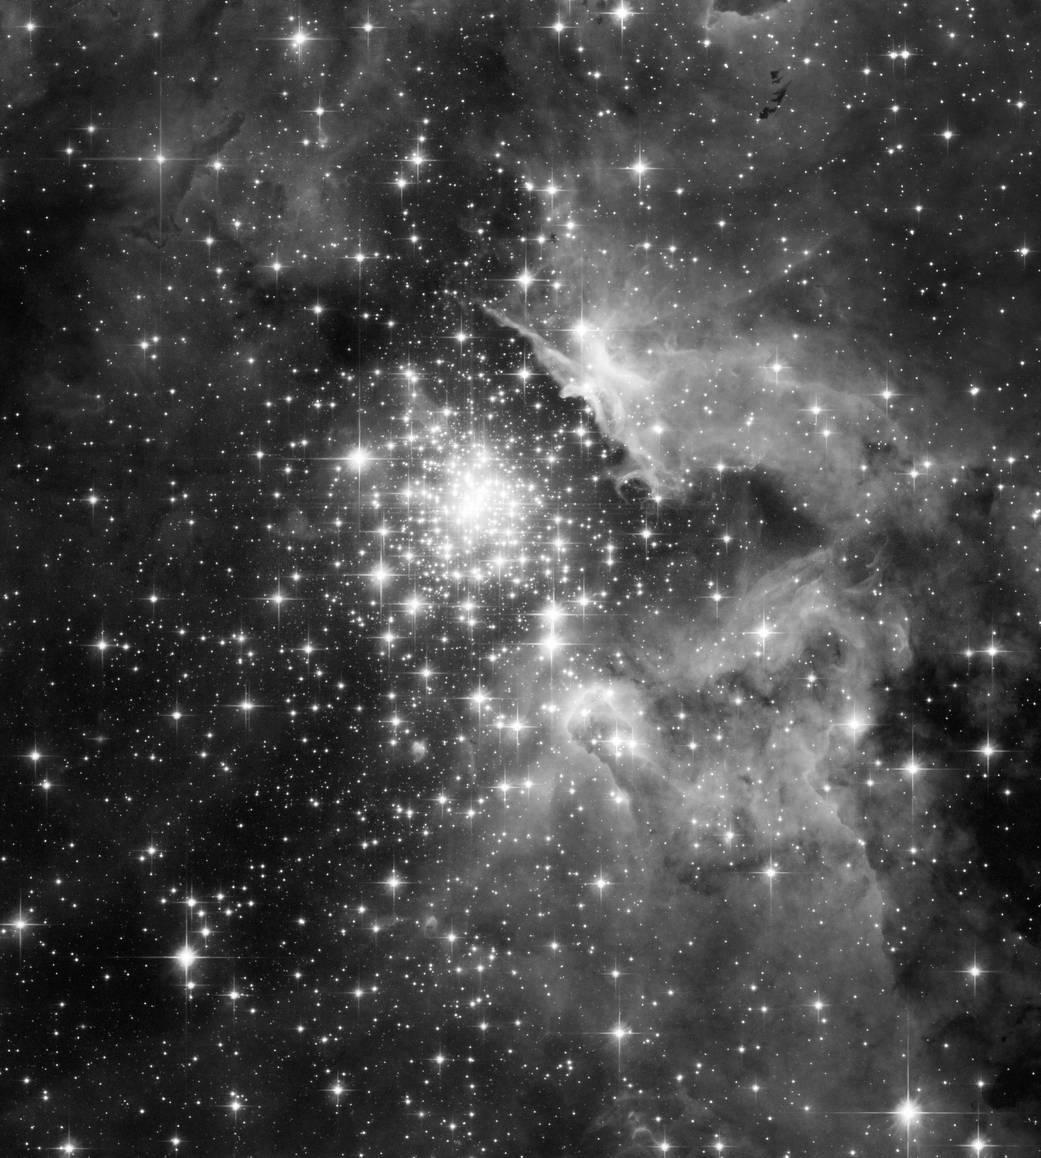
\includegraphics[height=5cm]{figures/hubble_gray.jpg}
    \caption{NGC 3603 (Hubble Space Telescope).}
    \label{fig:hubble-original-gray}
\end{subfigure}
%
\begin{subfigure}{.49\textwidth}
    \centering
    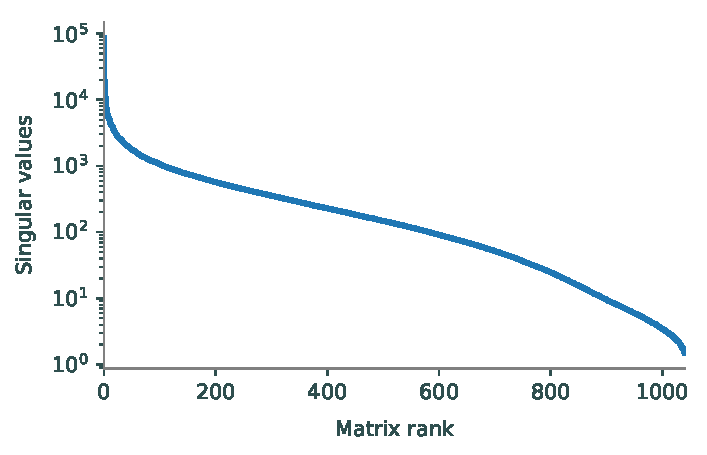
\includegraphics[width=\linewidth]{figures/hubble_svals.pdf}
    \caption{Singular values on a log scale.}
    \label{fig:hubble-log-svals}
\end{subfigure}
\caption{}
\label{fig:hubble}
\end{figure}

Figure \ref{fig:hubble-svd-rank-approximations} shows several low-rank approximations of the image in Figure \ref{fig:hubble-original-gray}.
Even at a low rank the image is recognizable.
By rank $120$, the approximation differs very little from the original.

\begin{figure}[H]
\centering
\begin{subfigure}{.32\textwidth}
    \centering
    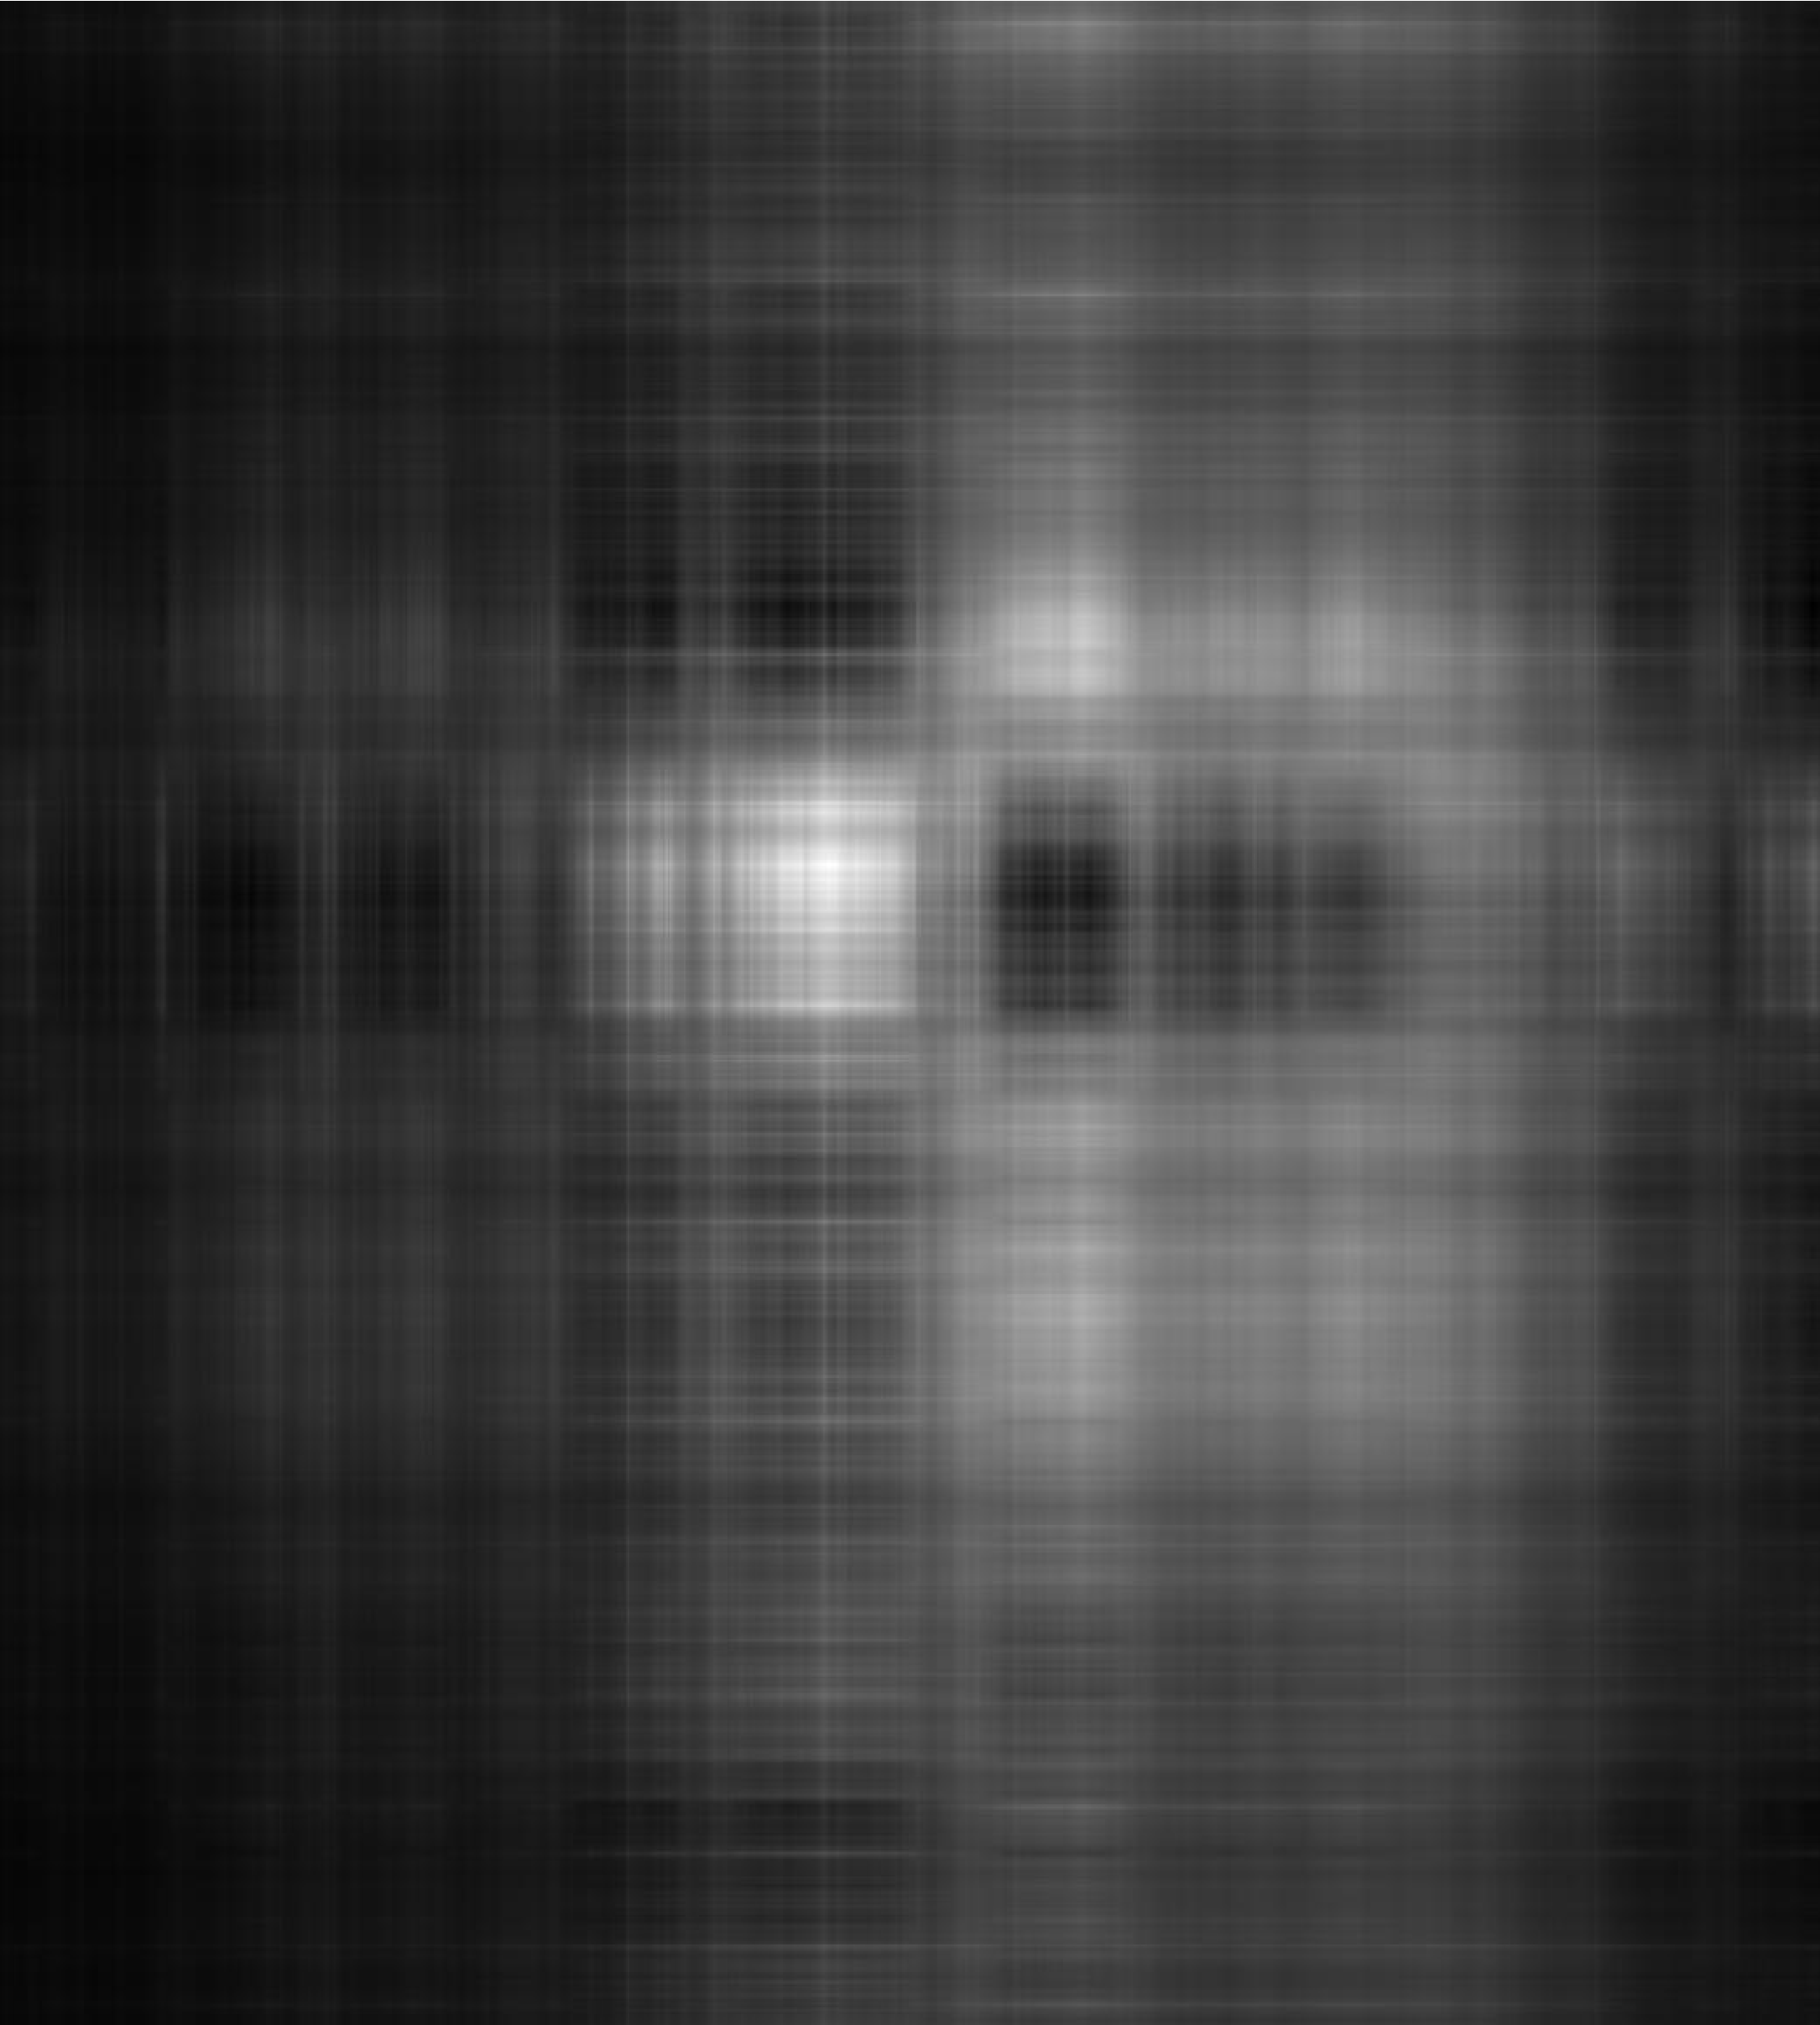
\includegraphics[width=\textwidth]{figures/rank2.pdf}
    \caption{Rank 2}
\end{subfigure}
%
\begin{subfigure}{.32\textwidth}
    \centering
    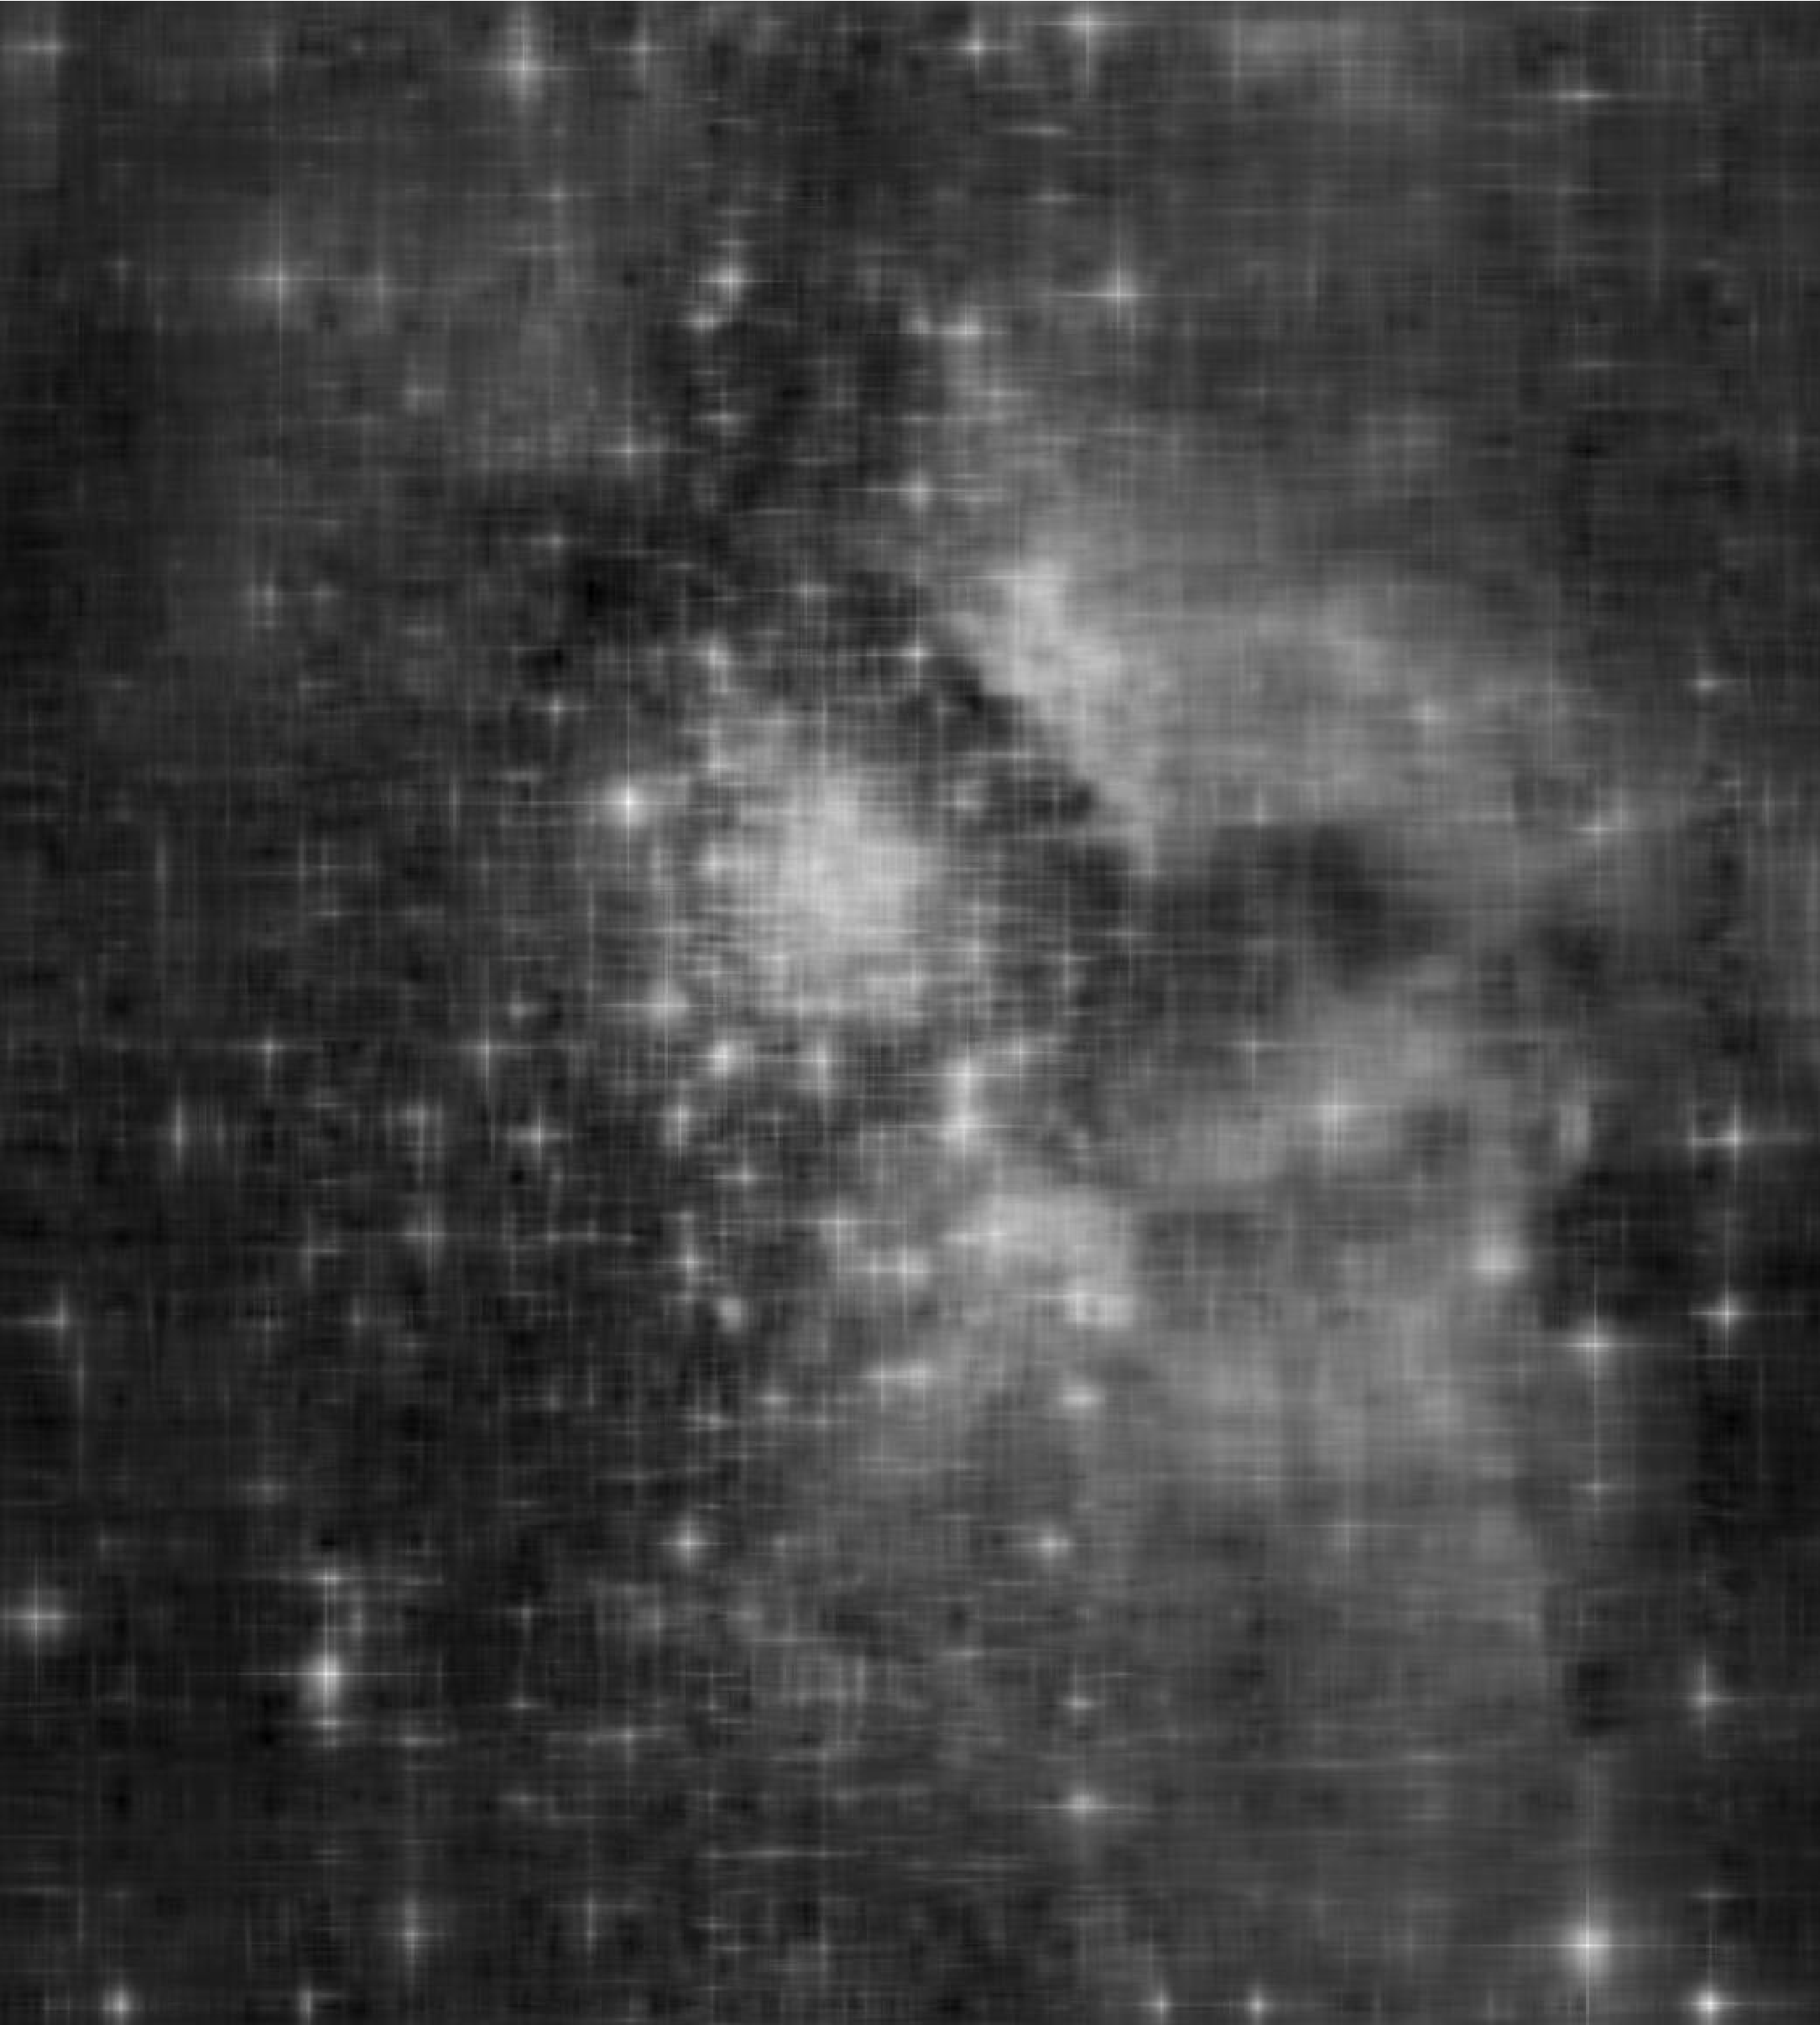
\includegraphics[width=\textwidth]{figures/rank20.pdf}
    \caption{Rank 20}
    \label{fig:hubble-rank20-approximation}
\end{subfigure}
%
\begin{subfigure}{.32\textwidth}
    \centering
    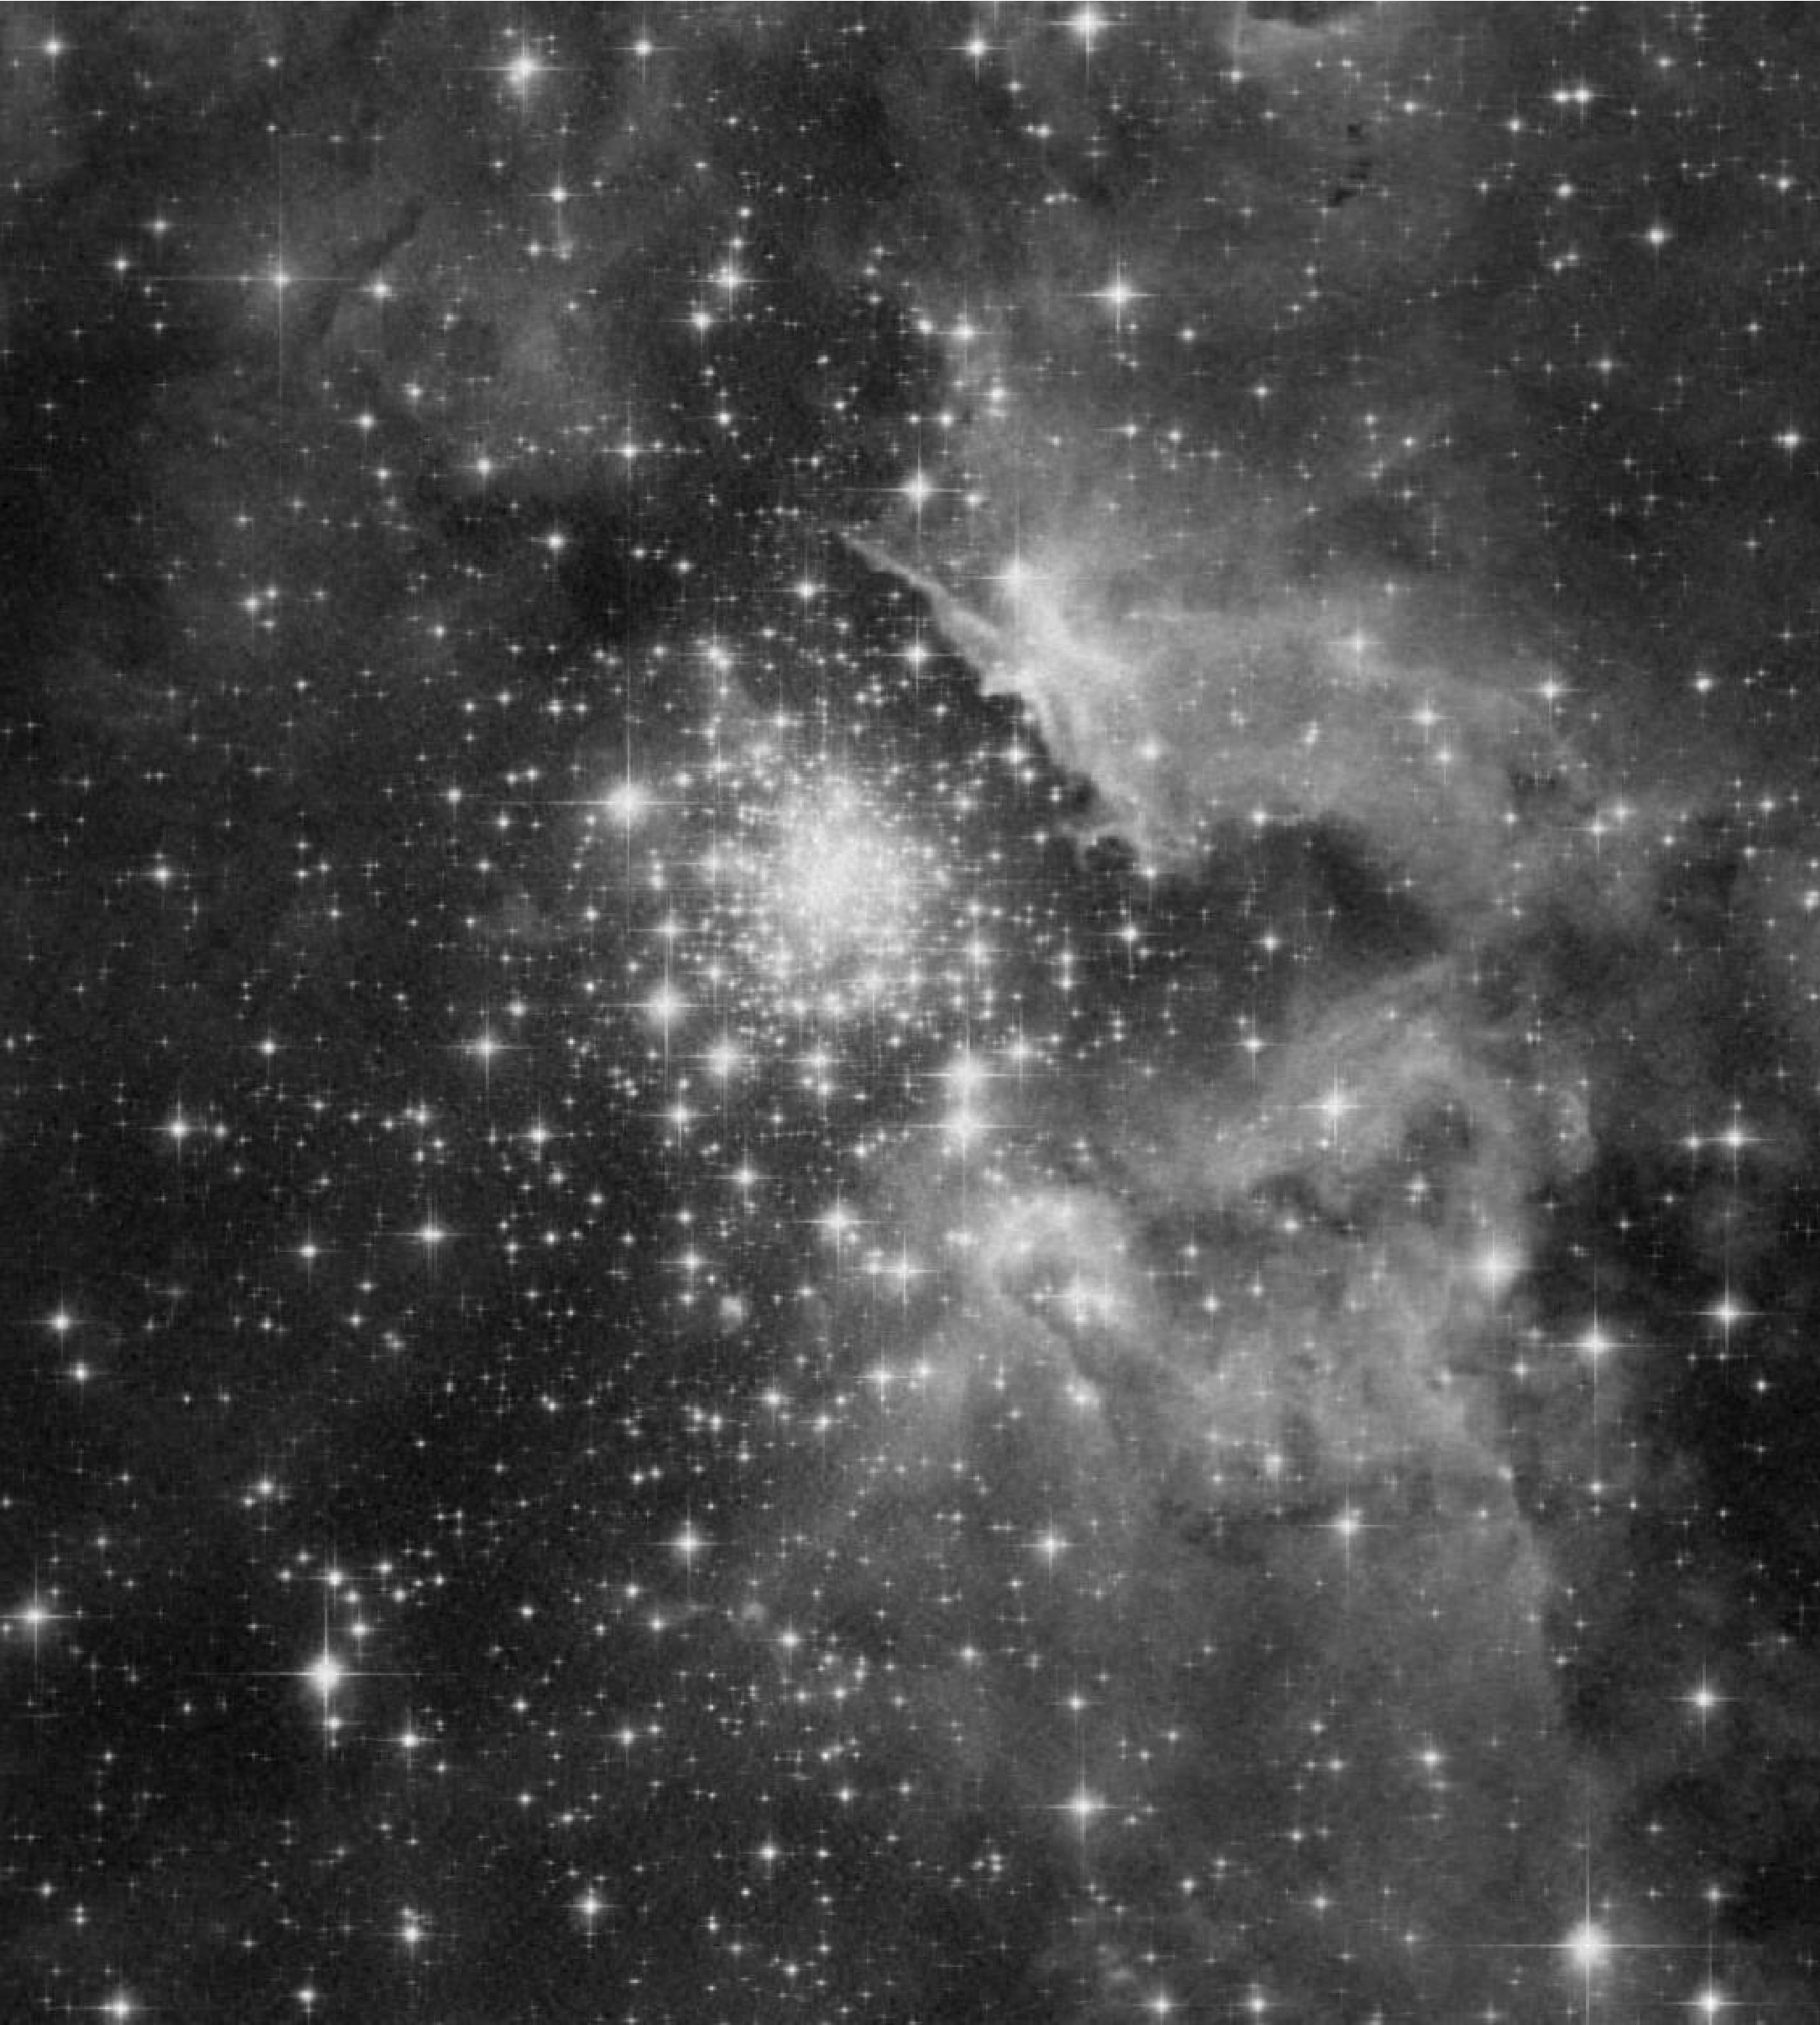
\includegraphics[width=\textwidth]{figures/rank120.pdf}
    \caption{Rank 120}
\end{subfigure}
\caption{}
\label{fig:hubble-svd-rank-approximations}
\end{figure}

Grayscale images are stored on a computer as 2-dimensional arrays, while color images are stored as 3-dimensional arrays---one layer each for red, green, and blue arrays.
To read and display images, use \li{imageio.imread()} and \li{plt.imshow()}.
Images are read in as integer arrays with entries between 0 and 255 (\li{dtype=np.uint8}), but \li{plt.imshow()} works better if the image is an array of floats in the interval $[0,1]$.
Scale the image properly by dividing the array by $255$.

\begin{lstlisting}
>>> from imageio import imread
>>> from matplotlib import pyplot as plt

# Send the RGB values to the interval (0,1).
>>> image_gray = imread("hubble_gray.jpg") / 255.
>>> image_gray.shape            # Grayscale images are 2-d arrays.
(1158, 1041)
>>> image_color = imread("hubble.jpg") / 255.
>>> image_color.shape           # Color images are 3-d arrays.
(1158, 1041, 3)

# The final axis has 3 layers for red, green, and blue values.
>>> red_layer = image_color[:,:,0]
>>> red_layer.shape
(1158, 1041)

# Display a gray image.
>>> plt.imshow(red_layer, cmap="gray")
>>> plt.axis("off")             # Turn off axis ticks and labels.
>>> plt.show()

# Display a color image.
>>> plt.imshow(image_color)     # cmap=None by default.
>>> plt.axis("off")
>>> plt.show()
\end{lstlisting}

\begin{problem} % Image compression.
Write a function that accepts the name of an image file and an integer $s$.
Use your function from Problem \ref{prob:svd_approx}, to compute the best rank-$s$ approximation of the image.
Plot the original image and the approximation in separate subplots.
In the figure title, report the difference in number of entries required to store the original image and the approximation (use \li{plt.suptitle()}).

Your function should be able to handle both grayscale and color images.
Read the image in and check its dimensions to see if it is color or not.
Grayscale images can be approximated directly since they are represented by 2-dimensional arrays.
For color images, let $R$, $G$, and $B$ be the matrices for the red, green, and blue layers of the image, respectively.
Calculate the low-rank approximations $R_s$, $G_s$, and $B_s$ separately, then put them together in a new 3-dimensional array of the same shape as the original image.
\\ (Hint: \li{np.dstack()} may be useful for putting the color layers back together.)

Finally, it is possible for the low-rank approximations to have values slightly outside the valid range of RGB values.
Set any values outside of the interval $[0,1]$ to the closer of the two boundary values.
\\ (Hint: fancy indexing and/or \li{np.clip()} may be useful here.)

To check, compressing \texttt{hubble\_gray.jpg} with a rank $20$ approximation should appear similar to Figure \ref{fig:hubble-rank20-approximation} and save $1,161,478$ matrix entries.
\end{problem}

% NOTE: we used to use A.nbytes instead of A.size to measure the reduction,
% but when images (dtype=np.uint8) are converted to float arrays
% (dtype=np.float64), the resulting arrays take much more memory to store, so =
% reporting the number of bytes saved often ends up being bigger than the
% original picture.

\newpage

\section*{Additional Material} % ==============================================

\subsection*{More on Computing the SVD} % -------------------------------------

For an $m\times n$ matrix $A$ of rank $r < \min\{m,n\}$, the compact SVD of $A$ neglects last $m-r$ columns of $U$ and the last $n-r$ columns of $V$.
The remaining columns of each matrix can be calculated by using Gram-Schmidt orthonormalization.
If $m < r < n$ or $n < r < m$, only one of $U_1$ and $V_1$ will need to be filled in to construct the full $U$ or $V$.
Computing these extra columns is one way to obtain a basis for $\mathscr{N}(A\hrm)$ or $\mathscr{N}(A)$.

Algorithm \ref{alg:compact-svd} begins with the assumption that we have a way to compute the eigenvalues and eigenvectors of $A\hrm A$.
Computing eigenvalues is a notoriously difficult problem, and computing the SVD from scratch without an eigenvalue solver is much more difficult than the routine described by Algorithm \ref{alg:compact-svd}.
The procedure involves two phases:
\begin{enumerate}
    \item Factor $A$ into $A = U_a B V\hrm_a$ where $B$ is bidiagonal (only nonzero on the diagonal and the first superdiagonal) and $U_a$ and $V_a$ are orthonormal.
    This is usually done via \emph{Golub-Kahan Bidiagonalization}, which uses Householder reflections, or \emph{Lawson-Hanson-Chan bidiagonalization}, which relies on the QR decomposition.
    \item Factor $B$ into $B = U_b \Sigma V\hrm_b$ by the QR algorithm or a divide-and-conquer algorithm.
    Then the SVD of $A$ is given by $A = (U_aU_b)\Sigma (V_aV_b)\hrm$.
\end{enumerate}
For more details, see Lecture 31 of \cite{Trefethen1997} or Section 5.4 of \emph{Applied Numerical Linear Algebra} by James W. Demmel.

\subsection*{Animating Images with Matplotlib} % ------------------------------

Matplotlib can be used to animate images that change over time.
For instance, we can show how the low-rank approximations of an image change as the rank $s$ increases, showing how the image is recovered as more ranks are added.
Try using the following code to create such an animation.

\begin{lstlisting}
from matplotlib import pyplot as plt
from matplotlib.animation import FuncAnimation

def animate_images(images):
    """Animate a sequence of images. The input is a list where each
    entry is an array that will be one frame of the animation.
    """
    fig = plt.figure()
    plt.axis("off")
    im = plt.imshow(images[0], animated=True)

    def update(index):
        plt.title("Rank {} Approximation".<<format>>(index))
        im.set_array(images[index])
        return im,              # Note the comma!

    a = FuncAnimation(fig, update, frames=len(images), blit=True)
    plt.show()
\end{lstlisting}
See \url{https://matplotlib.org/examples/animation/dynamic_image.html} for another example.
